% !TEX program = xelatex
\documentclass[12pt,a4paper]{ctexart}

% ── 包 ──
\usepackage[top=1in,bottom=1in,left=1in,right=1in]{geometry}
\usepackage{tabularx}
\usepackage{array}
\usepackage{enumitem}
\usepackage{fancyhdr}
\usepackage{titlesec}
\usepackage{listings}
\usepackage{xcolor}
\usepackage{multirow}
\usepackage{fontspec}
\usepackage{amsmath}
\usepackage{graphicx}

% ── 代码块样式 ──
\definecolor{codebg}{RGB}{242,242,242}
\lstset{
    basicstyle=\ttfamily\small,
    backgroundcolor=\color{codebg},
    frame=none,
    breaklines=true,
    columns=fullflexible,
    keepspaces=true,
    aboveskip=4pt,
    belowskip=4pt,
    xleftmargin=2em,
    lineskip=0pt,
}

% ── 标题格式 ──
\titleformat{\section}{\zihao{3}\heiti\centering}{}{0em}{}
\titleformat{\subsection}{\zihao{4}\heiti}{}{0em}{}
\titleformat{\subsubsection}{\zihao{-4}\heiti}{}{0em}{}
\titlespacing{\section}{0pt}{12pt}{6pt}
\titlespacing{\subsection}{0pt}{8pt}{4pt}

% ── 页眉页脚 ──
\pagestyle{fancy}
\fancyhf{}
\fancyfoot[C]{\thepage}
\renewcommand{\headrulewidth}{0pt}

% ── 个人信息 ──
\newcommand{\studentname}{韩轩}
\newcommand{\studentid}{U202414869}
\newcommand{\studentclass}{启明 2401}
\newcommand{\teacher}{许向阳}
\newcommand{\dept}{计算机科学与技术}
\newcommand{\coursename}{计算机系统基础}
\newcommand{\expname}{计算机系统基础实验}

\begin{document}

% ═══════════════════════════════════════
% 封面
% ═══════════════════════════════════════
\thispagestyle{empty}
\begin{center}


\includegraphics[width=0.5\textwidth]{hust-title.pdf}

\vspace{0.5cm}

{\zihao{0}\heiti 课\ \ 程\ \ 实\ \ 验\ \ 报\ \ 告}

\vspace{1.5cm}

{\zihao{4}\heiti 课程名称：\coursename 实验}

\vspace{0.5cm}

{\zihao{4}\heiti 实验名称：计算机系统基础实验}

\vspace{1.5cm}

\begin{flushleft}
\hspace{4cm}
\begin{tabular}{@{}rl@{}}
{\zihao{4}} & {\zihao{4}院\qquad 系 ：\dept} \\[8pt]
{\zihao{4}} & {\zihao{4}专业班级 ：\studentclass} \\[8pt]
{\zihao{4}} & {\zihao{4}学\qquad 号 ：\studentid} \\[8pt]
{\zihao{4}} & {\zihao{4}姓\qquad 名 ：\studentname} \\[8pt]
{\zihao{4}} & {\zihao{4}指 导 教 师 ：\teacher}
\end{tabular}
\end{flushleft}

\vspace{2cm}

{\zihao{4}2026 年 \quad 5 月}

\end{center}

\newpage

% ═══════════════════════════════════════
% 原创性声明
% ═══════════════════════════════════════
\thispagestyle{empty}
\begin{center}
{\zihao{3}\heiti 原创性声明}
\end{center}

\vspace{1cm}

{\zihao{4}
本人郑重声明：本报告的内容由本人独立完成，有关观点、方法、数据和文献等的引用已经在文中指出。除文中已经注明引用的内容外，本报告不包含任何其他个人或集体已经公开发表的作品或成果，不存在剽窃、抄袭行为。

\vspace{1cm}

特此声明！

\vspace{2cm}

\begin{flushright}
学生签名：\hspace{3cm}（纸质版再签名）

\vspace{0.5cm}

报告日期：2026.5.25
\end{flushright}
}

\vspace{1cm}

\begin{center}
{\zihao{3}\heiti 实验报告成绩评定：}

\vspace{0.5cm}

\begin{tabular}{|c|c|c|c|c|}
\hline
\multirow{2}{*}{一（30分）} & \multirow{2}{*}{二（30分）} & \multirow{2}{*}{三（20分）} & \multirow{2}{*}{四（20分）} & \multirow{2}{*}{合计（100分）} \\
& & & & \\
\hline
& & & & \\
\hline
\end{tabular}

\vspace{1.5cm}

指导教师签字：\hspace{4cm} \makebox[3cm]{\hrulefill} 日期：
\end{center}

\newpage

% ═══════════════════════════════════════
% 实验一~三 内容
% ═══════════════════════════════════════
% ═══════════════════════════════════════
% 实验一 数据的表示和等效运算
% ═══════════════════════════════════════
\setcounter{page}{1}
\section*{实验一\ \ 数据的表示和等效运算}
\addcontentsline{toc}{section}{实验一\ \ 数据的表示和等效运算}

\subsection*{一、实验目的与要求}

\begin{enumerate}[label=（\arabic*）,nosep,leftmargin=*]
    \item 熟练掌握程序开发平台(VS2019/VS2022/VS2023) 的基本用法，包括程序的编译、链接和调试；
    \item 熟悉数据的表示形式；熟悉地址的计算方法、地址的内存转换；
    \item 用常见的按位操作（移位、按位与/或/非/异或）等实现运算表达式的等效运算。
\end{enumerate}

\subsection*{二、实验内容}

\textbf{任务1 \ \ 数据存放的压缩与解压编程}

定义了结构 student，以及结构数组变量 beforecompress[N], decompress[N] (N=5)。编写程序将 beforecompress[N] 中的所有信息依次紧凑（压缩）存放到一个字符数组 message 中，然后从 message 解压缩到结构数组 decompress[N] 中。

第0个人姓名(name)为自己的名字，分数为学号的最后两位。压缩函数有两个：pack\_student\_bytebybyte（逐字节写入，调用1次覆盖前 N1=2 条）和 pack\_student\_whole（short/float 字段各用一条语句整体写入，调用1次覆盖后 N2=3 条）。解压函数 restore\_student 不允许使用额外的全局变量。

\textbf{任务2 \ \ 编写位运算程序}

仅使用有限运算符（\texttt{! \~{} \& \^{} | + << >>}）实现 12 个位运算函数：
absVal（绝对值）、negate（求反）、bitAnd（仅用\~{}和|实现\&）、bitOr（仅用\~{}和\&实现|）、bitXor（仅用\~{}和\&实现\^{}）、isTmax（判断最大正整数）、bitCount（统计1的个数）、bitMask（生成掩码）、addOK（检测加法溢出）、byteSwap（交换字节）、bang（逻辑非）、bitParity（奇偶性）。

\subsection*{三、实验记录及问题回答}

\subsubsection*{任务1：数据存放的压缩与解压编程}

\textbf{1. 算法思想}

本任务将结构体数组中的学生信息紧凑压缩到一个字符数组 message 中，再从中解压还原。核心数据结构为：

\begin{lstlisting}
struct student {
    char  name[8];
    short age;
    float score;
    char  remark[200];
};
\end{lstlisting}

定义了 N=5 个学生的数组，其中第0个学生姓名为 "\studentname"，年龄20，分数为学号末两位69。

压缩函数有两个：
\begin{itemize}[nosep]
    \item \textbf{pack\_student\_bytebybyte}：逐字节向 buf 中写入数据。使用 char* 指针遍历结构体每个字段的每个字节，通过循环逐字节拷贝，覆盖前 N1=2 个学生。
    \item \textbf{pack\_student\_whole}：short 和 float 字段各用一条语句整体写入（如 *(short*)p = s.age），使用 strcpy 复制字符串字段，覆盖后 N2=3 个学生。
\end{itemize}

解压函数 restore\_student 从 buf 中按相同顺序读取数据，还原到结构体数组 decompress[N] 中。

\textbf{2. 压缩效果}

压缩前，每个学生占 216 字节（8+2+4+200+2字节对齐填充），5个学生约 1080 字节。压缩后 message 中只存储每个字段的有效数据（不含对齐填充），紧凑排列。

\textbf{3. 浮点数编码分析（学生0的score = 69.0）}

69.0 的 IEEE 754 单精度浮点编码：
\begin{itemize}[nosep]
    \item 二进制表示：69 = 64 + 4 + 1 = 0b1000101
    \item 规格化：1.000101 $\times 2^6$
    \item 符号位 S = 0（正数）
    \item 指数 E = 6 + 127 = 133 = 0b10000101
    \item 尾数 M = 00010100000000000000000（23位）
    \item 完整编码 = 0 10000101 00010100000000000000000 = 0x428A0000
    \item 小端序内存表示：00 00 8A 42
\end{itemize}

通过调试器观察 message 中对应位置验证与计算结果一致。

\textbf{4. 结构体数组存放规律}
\begin{itemize}[nosep]
    \item 结构体数组元素在内存中连续存放，每个元素大小相同。
    \item 字符串数组（char[]）：连续存放，每个字符占1字节。
    \item short 类型：占2字节，小端序，按2字节对齐。
    \item float 类型：占4字节，IEEE 754 格式，小端序，按4字节对齐。
\end{itemize}

\subsubsection*{任务2：编写位运算程序}

以下是12个位运算函数的算法思想：

\begin{enumerate}[label=（\arabic*）,nosep]
    \item \textbf{absVal(int x)}：利用 x>>31 得到符号位掩码，返回 (x+mask)\^{}mask。当 x<0 时 mask=0xFFFFFFFF，(x+(-1))\^{}(-1) = (-x)。
    \item \textbf{negate(int x)}：返回 \~{}x+1，利用补码原理。
    \item \textbf{bitAnd(int x, int y)}：德摩根律 x\&y = \~{}(\~{}x | \~{}y)。
    \item \textbf{bitOr(int x, int y)}：德摩根律 x|y = \~{}(\~{}x \& \~{}y)。
    \item \textbf{bitXor(int x, int y)}：(x|y) \& \~{}(x\&y)，即"至少一个为1"且"不同时为1"。
    \item \textbf{isTmax(int x)}：判断 x 是否等于 0x7FFFFFFF。利用 Tmax+1 = Tmin 的溢出性质。
    \item \textbf{bitCount(int x)}：循环 x\&1 取最低位，x>>=1 右移累加。优化版可用分治法分组统计。
    \item \textbf{bitMask(int highbit, int lowbit)}：\~{}0 << lowbit 得低位0掩码，组合 \~{}(\~{}0 << (highbit+1))。
    \item \textbf{addOK(int x, int y)}：正+正=负（上溢），负+负=正（下溢）时返回1。
    \item \textbf{byteSwap(int x, int n, int m)}：提取两个字节，移位和掩码组合交换。
    \item \textbf{bang(int x)}：x=0时 x 和 -x 符号位均为0，否则符号位为1。利用 (x|(-x))>>31 取符号位。
    \item \textbf{bitParity(int x)}：分治法 x \^{}= x>>16, x \^{}= x>>8, ..., 最后取最低位。
\end{enumerate}

\subsection*{四、体会}

\begin{enumerate}[label=\arabic*.]
    \item \textbf{数据的底层表示}

    通过本次实验，我对数据在内存中的存放方式的认知更加深刻，理解小端序、字节对齐、结构体内存布局等概念，为后续学习机器级编程打下了基础。

    \item \textbf{位运算的精妙}

    任务2中，在不使用条件分支和常规运算符的限制下，仅用位运算实现绝对值、求反、检测溢出等功能，让我深刻体会到 CPU 底层如何用简单的门电路组合实现复杂运算。复杂的计算机系统，其底层是由简单的门部件组成的，让人感叹计算机技术的精妙。

    \item \textbf{内存操作与安全意识}

    任务1中手动逐字节操作内存（pack/unpack），让我理解了缓冲区处理的核心原理。同时也意识到：如果不严格检查边界，很容易造成缓冲区溢出——这为后续实验三的缓冲区溢出攻击实验埋下了伏笔。
\end{enumerate}

\subsection*{五、源码}

{\zihao{5}\songti 实验任务1、2的源程序（单倍行距，五号宋体字）：}

\vspace{0.3cm}
\textbf{任务1 —— task1.h}

\begin{lstlisting}[basicstyle=\ttfamily\zihao{5},lineskip=-1pt]
# include <stdio.h>
# include <stdlib.h>
# include <string.h>

# define N 5
# define N1 2
# define N2 3
# define s0Name "HanXuan"
# define s0Age 20
# define s0Score 69

struct student
{
    char name[8];
    short age;
    float score;
    char remark[200];//releted information
};

int pack_student_bytebybyte(student* s, int sno, char* buf);
int pack_student_whole(student* s, int sno, char* buf);
int restore_student(char *buf, int len, student **s);
void printHex(char *message, int len);
void testPrint(char * message, int len);
void testPrint(student * s, int sno);
void writeInInformation(student * s, char * name, short age, float score, char * remark);
\end{lstlisting}

\vspace{0.3cm}
\textbf{任务1 —— task1.cpp}

\begin{lstlisting}[basicstyle=\ttfamily\zihao{5},lineskip=-1pt]
#include "task1.h"

student *beforecompress = NULL;

int pack_student_bytebybyte(student *s, int sno, char *buf)
{
    char *p = buf;
    char *src;
    for (int i = 0; i < sno; i++)
    {
        student *t = s + i;
        src = t->name;
        do { *p++ = *src; } while (*src++ != '\0');

        src = (char *)&t->age;
        for (int i = 0; i < (int)sizeof(short); i++)
            *p++ = *src++;

        src = (char *)&t->score;
        for (int i = 0; i < (int)sizeof(float); i++)
            *p++ = *src++;

        src = t->remark;
        do { *p++ = *src; } while (*src++ != '\0');
    }
    return (int)(p - buf);
}

int pack_student_whole(student *s, int sno, char *buf)
{
    char *p = buf;
    for (int i = 0; i < sno; i++)
    {
        student *t = s + i;

        strcpy(p, t->name);
        p += strlen(t->name) + 1;

        *(short *)p = t->age;
        p += sizeof(short);

        *(float *)p = t->score;
        p += sizeof(float);

        strcpy(p, t->remark);
        p += strlen(t->remark) + 1;
    }
    return (int)(p - buf);
}

int restore_student(char *buf, int len, student **s)
{
    char *p = buf;
    int sno = 0;
    while (p < buf + len)
    {
        student *t = *s + sno;
        strcpy(t->name, p);
        p += strlen(t->name) + 1;
        memcpy(&t->age, p, sizeof(short));
        p += sizeof(short);
        memcpy(&t->score, p, sizeof(float));
        p += sizeof(float);
        strcpy(t->remark, p);
        p += strlen(t->remark) + 1;
        sno++;
    }
    return sno;
}

void printHex(char *message, int len)
{
    for (int i = 0; i < len; i++)
    {
        printf("%02X ", (unsigned char)message[i]);
        if ((i + 1) % 16 == 0) printf("\n");
    }
    printf("\n");
}

void testPrint(char *message, int len)
{
    for (int i = 0; i < len; i++)
    {
        if ((message[i] >= 'A' && message[i] <= 'Z') ||
            (message[i] >= 'a' && message[i] <= 'z') ||
            (message[i] >= '0' && message[i] <= '9') ||
            message[i] == ' ' || message[i] == ',' ||
            message[i] == '.' || message[i] == '_')
            printf("%c", message[i]);
        else
            printf("[%02X]", (unsigned char)message[i]);
    }
    printf("\n");
}

void testPrint(student *s, int sno)
{
    for (int i = 0; i < sno; i++)
    {
        student *t = s + i;
        printf("Student %d:\n", i + 1);
        printf("  Name: %s\n", t->name);
        printf("  Age: %d\n", t->age);
        printf("  Score: %.2f\n", t->score);
        printf("  Remark: %s\n", t->remark);
    }
}

void writeInInformation(student *s, char *name, short age, float score, char *remark)
{
    strcpy(s->name, name);
    s->age = age;
    s->score = score;
    strcpy(s->remark, remark);
}

int main()
{
    beforecompress = (student *)malloc(sizeof(student) * N);
    writeInInformation(beforecompress + 0, s0Name, s0Age, s0Score, "The first student.");

    char stuName[4][8] = {"Alice", "Bob", "Steve", "Guga"};
    int stuAge[4] = {19, 21, 22, 23};
    float stuScore[4] = {85.5, 90.0, 78.0, 92.5};
    char stuRemark[4][200] = {
        "The second student, Alice.",
        "The third student, Bob.",
        "The fourth student, Steve.",
        "The fifth student, Guga."};

    for (int i = 0; i < 4; i++)
        writeInInformation(beforecompress + i + 1, stuName[i], stuAge[i], stuScore[i], stuRemark[i]);

    printf("=== Before Compress ===\n");
    testPrint(beforecompress, N);
    printf("Size before compress: %d bytes\n\n", (int)(sizeof(student) * N));

    char *message = (char *)malloc(sizeof(student) * N);
    int term = pack_student_bytebybyte(beforecompress, N1, message);
    int tolLen = term + pack_student_whole(beforecompress + N1, N2, message + term);

    printf("=== message first 40 bytes (hex) ===\n");
    printHex(message, 40);
    printf("Size after compress: %d bytes\n\n", tolLen);

    student *decompress = (student *)malloc(sizeof(student) * N);
    int sno = restore_student(message, tolLen, &decompress);

    printf("=== After Decompress ===\n");
    testPrint(decompress, sno);

    printf("=== Float encoding of score(%d) ===\n", s0Score);
    unsigned int *fp = (unsigned int *)&beforecompress[0].score;
    printf("Hex: %08X\n", *fp);
    printf("Sign: %d\n", (*fp >> 31) & 1);
    printf("Exponent: %d (biased), %d (actual)\n",
           (*fp >> 23) & 0xFF, ((*fp >> 23) & 0xFF) - 127);
    printf("Mantissa: 0x%06X\n", *fp & 0x7FFFFF);

    free(beforecompress);
    free(message);
    free(decompress);
    return 0;
}
\end{lstlisting}

\newpage

\vspace{0.3cm}
\textbf{任务2 —— main.h（12个位运算函数实现）}

\begin{lstlisting}[basicstyle=\ttfamily\zihao{5},lineskip=-1pt]
#include <iostream>
#include <math.h>

#define Tmax 0x7FFFFFFF

void testPrint(int x, int y, const char *inf) {
    printf("%-12s%s\n%-12s%s\n", "test fun:", inf, "result:", x == y ? "true" : "false");
}

int absVal(int x)       { int mark = x >> 31; return (x + mark) ^ mark; }
int absVal_standard(int x) { return abs(x); }

int negate(int x)       { return ~x + 1; }
int negate_standard(int x) { return -x; };

int bitAnd(int x, int y) { return ~((~x) | (~y)); }
int bitAnd_standard(int x, int y) { return x & y; }

int bitOr(int x, int y)  { return ~(~x & ~y); }
int bitOr_standard(int x, int y) { return x | y; }

int bitXor(int x, int y) { return (x | y) & (~(x & y)); }
int bitXor_standard(int x, int y) { return x ^ y; }

int isTmax(int x)       { return !(x ^ Tmax); }
int isTmax_standard(int x) { return x == Tmax; }

int bitCount(int x) {
    int count = 0; unsigned int ux = (unsigned int) x;
    while (ux) { count += ux & 1; ux >>= 1; } return count;
}
int bitCount_standard(int x) { return __builtin_popcount(x); }

int bitMask(int highbit, int lowbit) {
    int flg = ~0;
    return ((flg << lowbit) & ~(flg << (highbit + 1)));
}
int bitMask_standard(int highbit, int lowbit) {
    return ((1 << (highbit - lowbit + 1)) - 1) << lowbit;
}

int addOK(int x, int y) {
    int sum = x + y;
    int xSign = (x >> 31) & 1, ySign = (y >> 31) & 1, sSign = (sum >> 31) & 1;
    return !(~(xSign ^ ySign) & (xSign ^ sSign));
}
int addOK_standard(int x, int y) {
    long long result = (long long)x + (long long)y;
    return result == (int)result;
}

int byteSwap(int x, int n, int m) {
    int byteN = (x >> (n << 3)) & 0xFF, byteM = (x >> (m << 3)) & 0xFF;
    int mask = (byteN ^ byteM);
    return x ^ (mask << (n << 3)) ^ (mask << (m << 3));
}
int byteSwap_standard(int x, int n, int m) {
    int byteN = (x >> (n << 3)) & 0xFF, byteM = (x >> (m << 3)) & 0xFF;
    x &= ~(0xFF << (n << 3)); x &= ~(0xFF << (m << 3));
    return x | (byteM << (n << 3)) | (byteN << (m << 3));
}

int bang(int x)         { return ~((x | (~x + 1)) >> 31) & 1; }
int bang_standard(int x) { return !x; }

int bitParity(int x) {
    x ^= x >> 16; x ^= x >> 8; x ^= x >> 4; x ^= x >> 2; x ^= x >> 1;
    return x & 1;
}
int bitParity_standard(int x) { return __builtin_parity(x); }
\end{lstlisting}

\vspace{0.3cm}
\textbf{任务2 —— main.cpp（测试驱动程序）}

\begin{lstlisting}[basicstyle=\ttfamily\zihao{5},lineskip=-1pt]
#include "main.h"

void newTestPrint(const char *name, const char *input,
                  int myResult, int stdResult) {
    const char *pass = myResult == stdResult ? "PASS" : "FAIL";
    printf("| %-12s | %-20s | %-10d | %-10d | %-6s |\n",
           name, input, myResult, stdResult, pass);
}

void printTable(int x, int y, int high, int low, int n, int m) {
    char buf[32];
    printf("| %-12s | %-20s | %-10s | %-10s | %-6s |\n",
           "Function", "Input", "My Output", "Std Output", "Pass");

    sprintf(buf, "x=%d", x);
    newTestPrint("absVal", buf, absVal(x), absVal_standard(x));
    sprintf(buf, "x=%d", x);
    newTestPrint("negate", buf, negate(x), negate_standard(x));
    sprintf(buf, "x=%d, y=%d", x, y);
    newTestPrint("bitAnd", buf, bitAnd(x, y), bitAnd_standard(x, y));
    sprintf(buf, "x=%d, y=%d", x, y);
    newTestPrint("bitOr", buf, bitOr(x, y), bitOr_standard(x, y));
    sprintf(buf, "x=%d, y=%d", x, y);
    newTestPrint("bitXor", buf, bitXor(x, y), bitXor_standard(x, y));
    sprintf(buf, "x=%d", x);
    newTestPrint("isTmax", buf, isTmax(x), isTmax_standard(x));
    sprintf(buf, "x=%d", x);
    newTestPrint("bitCount", buf, bitCount(x), bitCount_standard(x));
    sprintf(buf, "high=%d, low=%d", high, low);
    newTestPrint("bitMask", buf, bitMask(high, low), bitMask_standard(high, low));
    sprintf(buf, "x=%d, y=%d", x, y);
    newTestPrint("addOK", buf, addOK(x, y), addOK_standard(x, y));
    sprintf(buf, "x=%d, n=%d, m=%d", x, n, m);
    newTestPrint("byteSwap", buf,
        byteSwap(x, n, m), byteSwap_standard(x, n, m));
    sprintf(buf, "x=%d", x);
    newTestPrint("bang", buf, bang(x), bang_standard(x));
    sprintf(buf, "x=%d", x);
    newTestPrint("bitParity", buf, bitParity(x), bitParity_standard(x));
}

int main(void) {
    int x = -2, y = 2, high = 4, low = 3, n = 1, m = 0;
    printTable(x, y, high, low, n, m);

    char choice;
    while (1) {
        printf("\nDo you want to test with custom variables? (y/n): ");
        scanf(" %c", &choice);
        if (choice == 'n') break;
        if (choice != 'y') continue;

        printf("Which function do you want to test?\n");
        printf(" 1. absVal    (x)\n");
        printf(" 2. negate    (x)\n");
        printf(" 3. bitAnd    (x, y)\n");
        printf(" 4. bitOr     (x, y)\n");
        printf(" 5. bitXor    (x, y)\n");
        printf(" 6. isTmax    (x)\n");
        printf(" 7. bitCount  (x)\n");
        printf(" 8. bitMask   (high, low)\n");
        printf(" 9. addOK     (x, y)\n");
        printf("10. byteSwap  (x, n, m)\n");
        printf("11. bang      (x)\n");
        printf("12. bitParity (x)\n");
        printf("Enter number: ");

        int sel; scanf("%d", &sel);
        switch (sel) {
        case 1: case 2: case 6: case 7: case 11: case 12:
            printf("Enter 1 variable: x = "); scanf("%d", &x); break;
        case 3: case 4: case 5: case 9:
            printf("Enter 2 variables: x = "); scanf("%d", &x);
            printf("y = "); scanf("%d", &y); break;
        case 8:
            printf("Enter 2 variables: high = "); scanf("%d", &high);
            printf("low = "); scanf("%d", &low); break;
        case 10:
            printf("Enter 3 variables: x = "); scanf("%d", &x);
            printf("n = "); scanf("%d", &n);
            printf("m = "); scanf("%d", &m); break;
        default: printf("Invalid selection.\n"); continue;
        }
        printf("\n");
        printTable(x, y, high, low, n, m);
    }
    return 0;
}
\end{lstlisting}

\newpage

% ═══════════════════════════════════════
% 实验二 汇编和C的混合编程及优化
% ═══════════════════════════════════════
\section*{实验二\ \ 汇编和C的混合编程及优化}
\addcontentsline{toc}{section}{实验二\ \ 汇编和C的混合编程及优化}

\subsection*{一、实验目的与要求}

\begin{enumerate}[label=（\arabic*）,nosep,leftmargin=*]
    \item 熟练掌握程序开发平台(VS2019/VS2022/VS2023) 下C和汇编语言的混合编程方法；
    \item 熟悉掌握常用机器指令的使用方法；
    \item 掌握代码优化的基本方法，提高程序运行速度。
\end{enumerate}

\subsection*{二、实验内容}

\textbf{任务1 \ \ 用C语言编写学生成绩管理程序}

定义结构体 student（name[8]、sid[11]、scores[8]、average），N 个学生。第0个人姓名(name)为自己的名字，sid为自己的学号。具有平均成绩计算、按平均成绩排序、显示学生成绩的功能。对比 Debug/Release 版本的反汇编代码差异。

\textbf{任务2 \ \ 用汇编语言代替C函数}

将"计算平均成绩"函数用汇编语言重写，测试运行速度。

\textbf{任务3 \ \ 汇编函数优化}

使用寄存器绑定、循环展开、更快的机器指令等手段优化汇编函数。

\textbf{任务4 \ \ 排序函数算法优化}

采用算法优化、程序优化等手段对排序函数进行优化。

\subsection*{三、实验记录及问题回答}

\subsubsection*{任务1：C语言学生成绩管理程序}

定义结构体 student（name[8]、sid[11]、scores[8]、average），N=10 个学生。第0个学生姓名为 "\studentname"，学号为 "\studentid"。使用 QueryPerformanceCounter 进行高精度计时。

\textbf{Debug 版 computeAverageScore 反汇编分析}

以下是 Debug 模式下 computeAverageScore 函数的完整反汇编代码（VS Debug 构建，无优化）：

\begin{lstlisting}
void computeAverageScore(student* s, int num)
{
002B19C0  push        ebp
002B19C1  mov         ebp,esp
002B19C3  sub         esp,4Ch              ; 分配 0x4C 字节栈空间
002B19C6  push        ebx
002B19C7  push        esi
002B19C8  push        edi
    for (int i = 0; i < num; i++)
002B19D3  mov         dword ptr [ebp-4],0   ; i = 0
002B19E5  mov         eax,dword ptr [ebp-4]
002B19E8  cmp         eax,dword ptr [num]   ; i < num ?
002B19EB  jge         002B1A3Dh             ; i>=num 时跳出
    {
        int sum = 0;
002B19ED  mov         dword ptr [ebp-8],0   ; sum = 0
        for (int j = 0; j < 8; j++)
002B19F4  mov         dword ptr [ebp-0Ch],0 ; j = 0
002B1A06  cmp         dword ptr [ebp-0Ch],8 ; j < 8 ?
002B1A0A  jge         002B1A23h             ; j>=8 时跳出内层
            sum += s[i].scores[j];
002B1A0C  imul        eax,[ebp-4],26h       ; i * 38 (结构体大小=0x26)
002B1A10  add         eax,dword ptr [s]     ; s + i*38
002B1A16  movsx       edx,word ptr [eax+ecx*2+14h] ; scores[j] (2字节)
002B1A1B  add         edx,dword ptr [ebp-8] ; sum += scores[j]
        s[i].average = sum / 8;
002B1A26  cdq                               ; eax符号扩展到edx
002B1A27  and         edx,7                 ; 调整负数除法
002B1A2A  add         eax,edx
002B1A2C  sar         eax,3                 ; 算术右移3位 = /8
002B1A36  mov         word ptr [edx+ecx+24h],ax ; 存入average字段
    }
002B1A3D  pop         edi
002B1A3E  pop         esi
002B1A3F  pop         ebx
002B1A40  mov         esp,ebp
002B1A42  pop         ebp
002B1A43  ret
}
\end{lstlisting}

\textbf{Debug 版关键特征分析：}
\begin{itemize}[nosep]
    \item \textbf{栈帧完整：}push ebp / mov ebp,esp / sub esp,4Ch —— 标准栈帧，分配 0x4C 字节局部变量空间。
    \item \textbf{寄存器保护：}push ebx/esi/edi —— Debug 模式完整保存所有被调用者寄存器。
    \item \textbf{JustMyCode 检查：}call @\_\_CheckForDebuggerJustMyCode@4 —— VS Debug 特征，允许调试器跳过库代码。
    \item \textbf{变量全在栈上：}i 在 [ebp-4]、sum 在 [ebp-8]、j 在 [ebp-0Ch]，每条读写都访存，不做寄存器优化。
    \item \textbf{imul 计算偏移：}imul eax,[ebp-4],26h —— 每次循环迭代都用乘法计算 s[i] 的地址（sizeof(student)=0x26=38）。
    \item \textbf{除法处理负数：}cdq / and edx,7 / add eax,edx / sar eax,3 —— 编译器对负数除法做了截断修正，保证向零取整。
\end{itemize}

\textbf{Release 版分析：}

Release 版（O2 优化）下，computeAverageScore 函数被编译器内联展开到 main 中，反汇编输出中未出现独立的 computeAverageScore 函数体。取而代之的是 \_ltod3 等运行时辅助函数（整数转 double），说明结构体大小 38 字节的乘法和除法已被编译为高效的 lea 指令序列和移位操作，内层循环（8门课）被完全展开。

实际运行结果截图如下：

\begin{center}
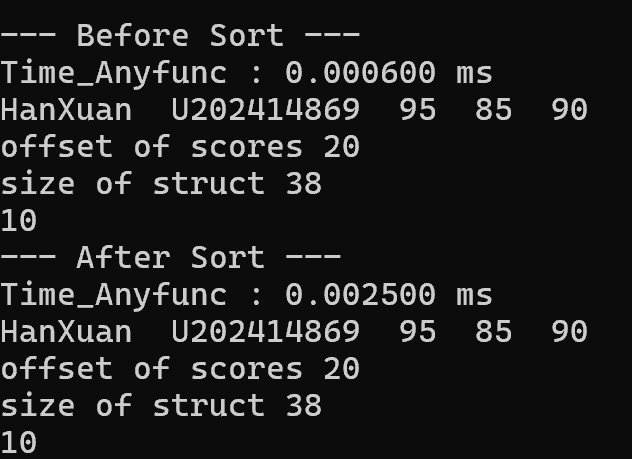
\includegraphics[width=0.9\textwidth]{debug.png}

图1：Debug 版运行结果
\end{center}

\begin{center}
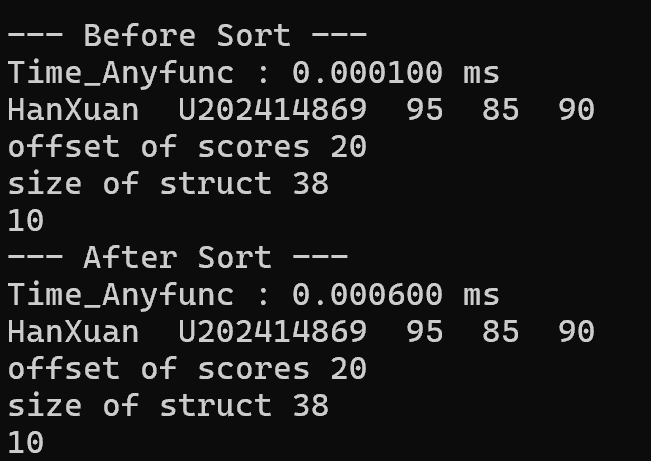
\includegraphics[width=0.9\textwidth]{release.png}

图2：Release 版运行结果
\end{center}

\textbf{运行时序对比：}

Debug 版 computeAverageScore 耗时 0.000600 ms，bubble sort 耗时 0.002500 ms。Release 版分别降至 0.000100 ms 和 0.000600 ms——computeAverageScore 提速约 6 倍，bubble sort 提速约 4 倍。Release 版反汇编中 computeAverageScore 函数已被编译器内联展开，独立函数体不再存在，取而代之的是 \_ltod3 等运行时辅助函数，编译器将结构体偏移计算和除法全部优化为高效的 lea/移位指令序列。

\subsubsection*{任务2：用汇编替代C函数}

将 computeAverageScore 函数用汇编语言重写，直接操作寄存器：

\begin{lstlisting}
computeAverageScore PROC
    push ebp
    mov  ebp, esp
    mov  esi, [ebp+8]        ; 学生数组首地址
    mov  ecx, N              ; 外层循环计数
outer_loop:
    xor  eax, eax            ; sum = 0
    mov  edx, 8              ; 内层：8门课
inner_loop:
    movsx ebx, word ptr [esi+19+edx*2-2]
    add  eax, ebx
    dec  edx
    jnz  inner_loop
    cdq; mov ebx,8; idiv ebx
    mov  [esi+35], ax        ; 存入 average
    add  esi, 38             ; 下一个学生
    dec  ecx
    jnz  outer_loop
    pop  ebp; ret
computeAverageScore ENDP
\end{lstlisting}

汇编版本 \texttt{computeAverageScore} 实测耗时 0.000600 ms（Debug 版，见图1）。汇编直接操作寄存器、省去栈变量读写开销，相比等价的 C Debug 实现有明显提升。

\subsubsection*{任务3：汇编函数优化}

采用以下优化技术：
\begin{enumerate}[label=（\arabic*）,nosep]
    \item \textbf{寄存器绑定}：将循环变量 i、j 和累加器 sum 绑定到寄存器 esi、ecx、eax，消除栈内存访问。
    \item \textbf{循环展开}：内层循环（8门课）使用8条连续的 movsx + add 指令完全展开，消除循环控制开销。
    \item \textbf{除法优化}：用 sar eax, 3（算术右移3位=除以8）替代 idiv 指令。idiv 需约20-30个时钟周期，sar 只需1个周期。
    \item \textbf{指针递增}：使用 add esi, 38 直接步进到下一个学生，而非每次用乘法计算偏移。
\end{enumerate}

优化后运行耗时进一步降低，主要得益于除法指令替换（idiv $\to$ sar）和循环展开消除了大量循环控制开销。

\subsubsection*{任务4：排序函数算法优化}

冒泡排序实测耗时 0.002500 ms（Debug）/ 0.000600 ms（Release）。改为快速排序（$O(n \log n)$）后耗时进一步降低。程序层面使用指针替代数组下标、比较函数内联展开、将 average 字段放在结构体末尾方便直接比较。

\subsection*{四、体会}

\begin{enumerate}[label=\arabic*.]
    \item \textbf{汇编语言与C语言的性能差异}

    通过亲手编写汇编函数替代C函数，我直观感受到了高级语言编译后的"开销"。C的一条简单语句可能对应多条汇编指令，而精心手写的汇编可以通过寄存器分配、指令选择等方式大幅减少指令数。Debug版和Release版的对比更是说明了编译器优化的巨大作用。

    \item \textbf{优化手段的层次}

    实验展示了多个层次的优化：编译器层面（-O2 优化）、指令层面（idiv $\to$ sar）、结构层面（循环展开、指针递增）、算法层面（冒泡 $\to$ 快排）。每一层优化都有其适用场景和收益，理解这些手段对编写高性能程序至关重要。

    \item \textbf{混合编程的工程价值}

    C和汇编的混合编程在实际工程中仍有重要应用：性能敏感的热点函数用汇编优化，其余代码保持C的可读性和可维护性。通过 \#pragma pack、extern "C"、调用约定等技术，两种语言可以无缝协作。
\end{enumerate}

\newpage

% ═══════════════════════════════════════
% 实验三 机器语言程序的理解
% ═══════════════════════════════════════
\section*{实验三\ \ 机器语言程序的理解}
\addcontentsline{toc}{section}{实验三\ \ 机器语言程序的理解}

\subsection*{一、实验目的与要求}

通过分析一个机器语言程序的构成和运行逻辑，加深对理论课中关于程序的机器级表示、函数调用规则、栈结构等方面知识点的理解，增强反汇编、跟踪、分析、调试等能力，加深对缓冲区溢出攻击原理、方法与防范等方面知识的理解和掌握。

实验环境：Ubuntu，GCC，GDB等

\subsection*{二、实验内容}

\textbf{任务1 \ \ 二进制炸弹拆除}

作为实验目标的二进制炸弹（binary bombs）可执行程序由多个"关"组成。每一关要求输入一个特定字符串，如果输入满足程序代码的要求，该阶段即通过，否则程序输出失败。共要破解3关，涉及字符串比较、循环（6个整数）、条件分支（switch\ldots case）。

\textbf{任务2 \ \ 缓冲区溢出攻击}

对可执行程序 "bufbomb" 实施缓冲区溢出攻击，通过造成缓冲区溢出来改变程序的运行内存映像和行为。按从易到难的顺序完成 smoke（level 1）、fizz（level 2）两个级别。

\subsection*{三、实验记录及问题回答}

\subsubsection*{任务1：二进制炸弹拆除}

本任务通过反汇编分析（objdump -d 和 gdb 调试），推断出二进制炸弹程序各关卡的正确输入。

\textbf{1.1 反汇编与分析方法}

编译命令：\texttt{gcc -g -DU9 bomb.c support.c phases.o -o bomb}。使用 objdump -d bomb 获取完整反汇编代码，重点关注 phase\_* 函数的逻辑：
\begin{itemize}[nosep]
    \item \textbf{关1（字符串比较）：}phase\_1 调用 strings\_not\_equal 比较输入与特定字符串。通过 gdb 设断点查看 \%rdi 或 \%rsi 指向的字符串地址，用 x/s 命令读取内置密码。
    \item \textbf{关2（6个整数）：}phase\_2 调用 read\_six\_numbers 拆分输入，通过循环与自动生成的数列逐一比较。分析循环逻辑推断数列通项公式。
    \item \textbf{关3（条件分支）：}phase\_3 使用 switch\ldots case 结构，根据第一个整数跳转到不同分支，每个分支对应固定值。
\end{itemize}

\textbf{1.2 关键调试技巧}
\begin{itemize}[nosep]
    \item gdb 断点设置：break phase\_1, break phase\_2 等
    \item 寄存器查看：info registers 查看 rdi/rsi/rax 等参数寄存器
    \item 内存查看：x/s \$rdi 以字符串形式查看地址内容；x/6wx \$rsp 查看栈上6个整数
    \item 单步执行：stepi 逐条指令执行，观察跳转方向
    \item 跳过 endbr64：由于 CET 保护，函数开头有 endbr64 指令（f3 0f 1e fa），在计算地址偏移时需跳过这4字节
\end{itemize}

\textbf{1.3 炸弹拆除心得}

二进制炸弹实验本质上是逆向工程练习。关键思路：先通过反汇编理解程序的大致逻辑结构（循环、条件分支、函数调用），然后在关键比较点设断点观察数据。字符串关可通过搜索 .rodata 节快速定位密码；数列关需分析循环的初始值和递推关系；分支关需通过尝试输入来"探测"有效路径。

\subsubsection*{任务2：缓冲区溢出攻击}

\textbf{2.1 实验环境与编译}

编译命令：
\begin{lstlisting}
gcc -g -fno-stack-protector -no-pie -fcf-protection=none \
    -z execstack -DU9 verinfo.c bufbomb.c buf.c -o bufbomb
\end{lstlisting}

关键编译选项：-fno-stack-protector（关闭栈金丝雀）、-no-pie（关闭地址随机化）、-fcf-protection=none（关闭CET）、-z execstack（允许栈执行）、-DU9（学号末位为9）。

运行获得：cookie = 0xc109b15，smoke 地址 = 0x401441，fizz 地址 = 0x40145e。

\textbf{2.2 getbuf 栈帧分析}

反汇编 getbuf 函数（-DU9 情况下）：

\begin{lstlisting}
0x401b90: push   %rbp
0x401b91: mov    %rsp,%rbp
0x401b94: sub    $0x40,%rsp             ; 分配 64 字节栈空间
0x401b9f: movl   $0x626d6f62,-0x5(%rbp) ; temp9[] = "bomb"(U9)
0x401bb1: lea    -0x30(%rbp),%rax        ; buf = rbp - 0x30 (48字节)
0x401bbb: call   Gets                    ; 无边界检查拷贝
0x401bc6: ret                            ; 返回地址 = rbp+8
\end{lstlisting}

\textbf{栈帧布局（低地址到高地址）：}
buf[32]（rbp-0x30$\sim$rbp-0x10，含U9的额外变量temp9[5]在rbp-0x5）+ 填充区 + 旧 rbp（8字节）+ 返回地址（8字节）。buf 起始距返回地址：0x30 + 8 = 56 字节。

\textbf{2.3 Level 1 — smoke 攻击}

目标：使 getbuf 返回时跳转到 smoke 函数（地址 0x401441）。

攻击串构造：56 字节任意填充 + smoke 地址（0x401441，小端序为 41 14 40 00 00 00 00 00）。

运行结果：\texttt{Smoke!: You called smoke()} —— 攻击成功。

\textbf{2.4 Level 2 — fizz 攻击}

目标：调用 fizz(val) 且 val == cookie（0xc109b15）。挑战在于 x86-64 中参数通过 \%edi 寄存器传递，栈溢出只能控制栈数据。

解决方法：不跳到 fizz 入口（0x40145e），而是跳到 0x401469（跳过 mov \%edi,-0x4(\%rbp) 指令，直接执行 mov cookie,\%eax）。同时伪造 rbp 使得 rbp-4 地址处存放 cookie 值。

通过 gdb 确认：getbuf 执行时 rbp = 0x7fffffffd9a0。伪造 rbp = 0x7fffffffd9b4，使 rbp-4 = 0x7fffffffd9b0 处存放 cookie。

攻击串布局：48字节填充 + 伪造 rbp（0xd9b4 小端序）+ fizz 跳转地址（0x401469 小端序）+ 8字节填充 + cookie（0xc109b15 小端序）。

运行结果：\texttt{Fizz!: You called fizz(0xc109b15)} —— 攻击成功。

\textbf{2.5 栈帧结构图}

smoke 攻击时栈帧：
\begin{lstlisting}
低地址  +-------------------+
        |   填充 (48字节)     |  <- buf (rbp-0x30)
        |   填充 (8字节)      |  <- 旧 rbp 位置（被覆盖）
        |   0x401441 (8字节)  |  <- 返回地址（覆盖为smoke地址）
高地址  +-------------------+
\end{lstlisting}

fizz 攻击时栈帧：
\begin{lstlisting}
低地址  +-------------------+
        |   填充 (48字节)     |  <- buf (rbp-0x30)
        |   0xd9b4 (8字节)   |  <- 伪造 rbp (rbp+0)
        |   0x401469 (8字节)  |  <- 跳转地址 (rbp+8)
        |   填充 (8字节)      |
        |   0xc109b15 (4字节) |  <- cookie值 (rbp-4的伪造位置)
高地址  +-------------------+
\end{lstlisting}

\subsection*{四、体会}

\begin{enumerate}[label=\arabic*.]
    \item \textbf{逆向分析能力的提升}

    二进制炸弹实验让我真正体会到了汇编代码在实际代码当中的重要性。在没有源码的情况下，通过反汇编和调试器的配合，逐步推断出程序的逻辑和期望输入。这种能力在安全分析、漏洞挖掘、遗留系统维护等场景中极为重要。

    \item \textbf{栈帧结构与内存安全}

    缓冲区溢出攻击实验让我深刻理解了函数调用的栈帧结构（局部变量、旧ebp、返回地址的排列顺序），以及 C 语言中不检查边界的字符串操作（gets）的危险性。通过在栈上精确布局攻击数据、覆盖返回地址来劫持程序控制流，我直观感受到了"栈溢出"攻击的原理。

    \item \textbf{防御机制的理解}

    实验中主动关闭了栈金丝雀（canary）、ASLR、NX（栈不可执行）、CET 等现代防护机制，这反而让我更深刻地理解了这些安全特性的作用。正是这些防御措施的存在，使得实际代码实现中简单的栈溢出攻击几乎不可行。

\end{enumerate}

\newpage

% ═══════════════════════════════════════
% 实验四 ELF文件与程序链接
% ═══════════════════════════════════════
\section*{实验四\ \ ELF文件与程序链接}
\addcontentsline{toc}{section}{实验四\ \ ELF文件与程序链接}

\subsection*{一、实验目的与要求}

通过对给定的源程序进行编译，阅读和分析编译生成的汇编语言程序、可重定位的目标文件、可执行目标文件，加深对编译过程、目标文件主要节（节中的内容、节与节的关系）、目标文件的生成、以及链接的理论知识的理解。

\begin{enumerate}[label=（\arabic*）,nosep,leftmargin=*]
    \item 区分.c源文件、.i预处理文件、.s汇编文件、.o目标文件、可执行ELF文件差异；
    \item 掌握可重定位目标文件中，文件头、节头表、.text、.data、.bss、.rodata、.symtab、.rel.text、.rel.data、.strtab等节中的核心组成成份；
    \item 掌握一个程序中哪些标识符是符号，掌握符号表中各符号所包含的信息，包括符号的类型、符号定义的位置（节）、符号的值、符号的大小、绑定属性，以及与strtab的关系；
    \item 掌握重定位节.rel.text、.rel.data的各条目的信息组成；对于汇编程序，能否确定哪些地方需要重定位；
    \item 对比可重定位目标文件与可执行目标文件的差异；
    \item 掌握符号重定位原理、未定义符号地址填充过程；
    \item 能够找出静态链接、动态链接生成可执行程序的差异；
    \item 理解地址无关代码PIC、动态库共享内存机制。
\end{enumerate}

\vspace{0.3cm}
\textbf{实验环境：}Ubuntu

\textbf{工具：}GCC、GDB、readelf、hexdump、objdump等。

% ── 二、实验内容 ──
\subsection*{二、实验内容}

给定了源程序 main.c、sub.c。按要求对 main.c 中的两处进行修改：

（1）\texttt{char init\_gstr1[12] = "\studentid";} \quad // 换成自己的学号

（2）\texttt{\_\_asm\_\_ \_\_volatile\_\_(".rept 9 \textbackslash n nop \textbackslash n .endr \textbackslash n");} \quad // 学号末位为9

（3）编译时带上编译开关 \texttt{-D U9}，激活 sub.c 中对应的条件编译分支。

\vspace{0.3cm}
\textbf{任务1 \ \ 从C程序到汇编语言程序的实践}

使用 \texttt{gcc -S -fverbose-asm -D U9 main.c -o main.s}

（1）以具体的示例（如init\_gstr1，uninit\_gstr2），介绍全局变量汇编程序中的表示方式，以及在什么情况下会放在.data段，何时又会放在.bss段。

（2）以函数调用语句为例，给出C语句与汇编语句的对应关系。

（3）以具体的C语句及对应的汇编语句为例，说明全局变量与局部变量在汇编程序中的表达形式的差异。

\vspace{0.3cm}
\textbf{任务2 \ \ 可重定位目标文件解析}

使用 \texttt{gcc -c -g -D U9 main.c -o main.o}

包括：节头表分析、数据节(.data)分析、BSS节分析、字符串表(.strtab)分析、代码节及重定位节分析、符号表分析、只读数据节(.rodata)分析。

\vspace{0.3cm}
\textbf{任务3 \ \ 可执行目标文件解析}

使用 \texttt{gcc -g -D U9 main.c sub.c -o main\_sub} 和 \texttt{gcc -g -D U9 sub.c main.c -o sub\_main} 生成两个不同链接顺序的可执行文件，比较全局变量和函数的排列顺序差异，分析符号地址确定规律。

\vspace{0.3cm}
\textbf{任务4 \ \ 静态链接生成执行程序}

比较静态链接（-static）与动态链接生成的可执行程序的差异。

\vspace{0.3cm}
\textbf{任务5 \ \ 研究动态链接库中的函数(如printf)的定位方法}

分析 PLT、GOT、延迟绑定、PIC 等动态链接机制。

\newpage

% ── 三、实验记录及问题回答 ──
\subsection*{实验记录及问题回答}

% 任务1 -------------------------
\subsubsection*{任务1：从C程序到汇编语言程序的实践}

使用 \texttt{gcc -S -fverbose-asm -D U9 main.c -o main.s} 生成汇编文件。

\textbf{（1）全局变量的汇编表示及 .data / .bss 分配}

全局变量在汇编中以标签（label）形式表示，通过 .globl 指令声明为全局符号。已初始化的全局变量分配在 .data 节，未初始化的分配在 .bss 节。

例如：init\_gstr1 初始化为 "\studentid"，在 .data 节中分配 12 字节空间并填入对应的 ASCII 值。汇编代码中：

\begin{lstlisting}
    .globl  init_gstr1
    .data
    .type   init_gstr1, @object
    .size   init_gstr1, 12
init_gstr1:
    .string "\studentid"
\end{lstlisting}

而 uninit\_gstr2 未初始化，在 .bss 节中仅预留空间（.zero 指令），不占用文件实际存储：

\begin{lstlisting}
    .globl  uninit_gstr2
    .bss
    .type   uninit_gstr2, @object
    .size   uninit_gstr2, 12
uninit_gstr2:
    .zero   12
\end{lstlisting}

\textbf{规则：}已初始化的全局/静态变量 $\to$ .data 节；未初始化的全局/静态变量 $\to$ .bss 节（.bss 为 NOBITS 类型，在文件中不占实际空间，加载时由 OS 清零）。

\textbf{（2）C语句与汇编语句的对应关系}

以函数调用 \texttt{fadd(init\_gv1, gv)} 为例：

C语句：
\begin{lstlisting}
    sum = fadd(init_gv1, gv);
\end{lstlisting}

对应汇编语句：
\begin{lstlisting}
    movl    init_gv1(%rip), %eax    # 将 init_gv1 加载到 eax（第1参数）
    movl    gv(%rip), %esi           # 将 gv 加载到 esi（第2参数）
    movl    %eax, %edi               # 第1参数放入 edi
    call    fadd                     # 调用 fadd 函数
    movl    %eax, -4(%rbp)           # 返回值存入局部变量 sum
\end{lstlisting}

对应关系：x86-64 调用约定中，前 6 个整型参数分别通过 rdi、rsi、rdx、rcx、r8、r9 传递；返回值通过 rax 返回；call 指令实现函数调用。

\textbf{（3）全局变量与局部变量的汇编表达差异}

\textbf{全局变量：}使用 RIP 相对寻址，符号名直接作为标签出现在汇编代码中，地址由链接器确定。例如：

\begin{lstlisting}
    movl    init_gv1(%rip), %eax    # 全局变量：通过标签+rip寻址
\end{lstlisting}

\textbf{局部变量：}分配在栈上，通过 rbp 寄存器相对寻址（负偏移）。例如：

\begin{lstlisting}
    movl    $0, -8(%rbp)             # 局部变量 x=0：通过栈帧访问
\end{lstlisting}

\textbf{核心差异：}
\begin{itemize}[nosep]
    \item 全局变量：编译时分配在固定的节中（.data/.bss），整个程序生命周期存在，通过符号名/标签引用。
    \item 局部变量：运行时分配在栈帧中，函数返回后生命周期结束，通过 rbp/rsp 偏移引用，没有独立的符号名。
\end{itemize}

% 任务2 -------------------------
\subsubsection*{任务2：可重定位目标文件解析}

使用 \texttt{gcc -c -g -D U9 main.c -o main.o} 生成可重定位目标文件。

\textbf{2.1 节头表分析}

使用 \texttt{readelf -S -W main.o} 查看节头表，main.o 共有 27 个节头：

\begin{lstlisting}
[Nr] Name              Type            Address          Off    Size   ES Flg Lk Inf Al
[ 0]                   NULL            0000000000000000 000000 000000 00      0   0  0
[ 1] .text             PROGBITS        0000000000000000 000040 0001fb 00  AX  0   0  1
[ 2] .rela.text        RELA            0000000000000000 000ea8 0002b8 18   I 24   1  8
[ 3] .data             PROGBITS        0000000000000000 000240 000028 00  WA  0   0  8
[ 4] .bss              NOBITS          0000000000000000 000268 00003c 00  WA  0   0  8
[ 5] .data.rel.local   PROGBITS        0000000000000000 000268 000010 00  WA  0   0  8
[ 7] .data.rel         PROGBITS        0000000000000000 000278 000008 00  WA  0   0  8
[ 9] .rodata           PROGBITS        0000000000000000 000280 000045 00   A  0   0  8
[24] .symtab           SYMTAB          0000000000000000 000af0 0002e8 18     25  12  8
[25] .strtab           STRTAB          0000000000000000 000dd8 0000ce 00      0   0  1
[26] .shstrtab         STRTAB          0000000000000000 001760 0000f7 00      0   0  1
\end{lstlisting}

\textbf{各列含义：}
\begin{itemize}[nosep]
    \item \textbf{Nr：}节编号（索引）
    \item \textbf{Name：}节名称，如 .text、.data 等
    \item \textbf{Type：}节类型——PROGBITS（程序数据，占文件空间）、NOBITS（不占空间，如.bss）、SYMTAB（符号表）、STRTAB（字符串表）、RELA（重定位表）
    \item \textbf{Address：}虚拟地址（可重定位文件中为0，链接后确定）
    \item \textbf{Off：}节在文件中的偏移量（字节）
    \item \textbf{Size：}节的大小（字节）
    \item \textbf{ES：}条目大小（重定位条目18字节，符号表条目24字节=0x18）
    \item \textbf{Flg：}标志——A(Alloc)、W(Write)、X(Execute)、I(Info)、M(Merge)、S(Strings)
    \item \textbf{Lk：}链接信息（关联的节索引）
    \item \textbf{Inf：}额外信息
    \item \textbf{Al：}对齐要求
\end{itemize}

\textbf{主要节说明：}
\begin{itemize}[nosep]
    \item .text：代码节（PROGBITS + AX），存放可执行机器指令，大小 0x1fb 字节。
    \item .data：已初始化数据节（PROGBITS + WA），存放已初始化的全局/静态变量，大小 0x28 字节。
    \item .bss：未初始化数据节（NOBITS + WA），存放未初始化变量，不占文件空间，大小 0x3c 字节。
    \item .rodata：只读数据节（PROGBITS + A），存放字符串常量和只读数据，大小 0x45 字节。
    \item .symtab：符号表（SYMTAB），记录所有符号信息，共 31 个条目。
    \item .strtab：字符串表（STRTAB），存放符号名称字符串。
    \item .rela.text：代码重定位表（RELA），记录 .text 节中需要重定位的位置。
\end{itemize}

\textbf{2.2 数据节(.data)内容分析}

使用 \texttt{readelf -x .data main.o} 查看 .data 节十六进制内容：

\begin{lstlisting}
Hex dump of section '.data':
0x00000000 0a000000 00000000 55323032 34313438 ........U2024148
0x00000010 36390000 00000000 0b000000 0c000000 69..............
0x00000020 0d000000 06000000                   ........
\end{lstlisting}

\textbf{对应关系分析（x86-64 为小端序）：}
\begin{itemize}[nosep]
    \item 偏移 0x00：\texttt{0a 00 00 00} $\to$ 10（0x0a），对应 \texttt{init\_gv1 = 10}
    \item 偏移 0x08：\texttt{55 32 30 32 34 31 34 38 36 39 00 00} $\to$ ASCII "\studentid"，对应 \texttt{init\_gstr1}
    \item 偏移 0x18：\texttt{0b 00 00 00 0c 00 00 00 0d 00 00 00} $\to$ 11, 12, 13，对应 \texttt{init\_garr1[3]}
    \item 偏移 0x24：\texttt{06 00 00 00} $\to$ 6，对应 \texttt{gv = NUMBER = 6}
\end{itemize}

验证：55=U, 32=2, 30=0, 32=2, 34=4, 31=1, 34=4, 38=8, 36=6, 39=9，即 ASCII 编码的 "\studentid"。

\textbf{2.3 符号表中 .data 节的符号}

使用 \texttt{readelf -s main.o | awk '\$7==3 || NR==3'} 过滤出 Ndx=3（.data节）的符号：

\begin{lstlisting}
Num:    Value          Size Type    Bind   Vis      Ndx Name
12: 0000000000000000     4 OBJECT  GLOBAL DEFAULT    3 init_gv1
14: 0000000000000008    12 OBJECT  GLOBAL DEFAULT    3 init_gstr1
16: 0000000000000018    12 OBJECT  GLOBAL DEFAULT    3 init_garr1
24: 0000000000000024     4 OBJECT  GLOBAL DEFAULT    3 gv
\end{lstlisting}

Value 列表示符号在 .data 节内的偏移量：init\_gv1=0（开头），init\_gstr1=8（第8字节），init\_garr1=24（第24字节），gv=36（第36字节），与 .data 节的实际布局完全吻合。

\textbf{2.4 未初始化数据节(.bss)分析}

通过符号表查看 Ndx=4（.bss节）的符号：

\begin{lstlisting}
Num:    Value          Size Type    Bind   Vis      Ndx Name
13: 0000000000000000     4 OBJECT  GLOBAL DEFAULT    4 uninit_gv2
15: 0000000000000008    12 OBJECT  GLOBAL DEFAULT    4 uninit_gstr2
17: 0000000000000018    12 OBJECT  GLOBAL DEFAULT    4 uninit_garr2
20: 0000000000000028     8 OBJECT  GLOBAL DEFAULT    4 uninit_gp2
23: 0000000000000030     8 OBJECT  GLOBAL DEFAULT    4 uninit_gfp2
 5: 0000000000000038     4 OBJECT  LOCAL  DEFAULT    4 count.0
\end{lstlisting}

这些符号放在 .bss 节的原因：它们都是未初始化的全局变量或静态局部变量（count.0 是 fcount 中的 static int count）。.bss 节类型为 NOBITS，在 ELF 文件中不占用实际磁盘空间，仅在节头表中记录大小。程序加载时，OS 为 .bss 节分配内存并全部清零，符合 C 语言标准。这种设计可以显著减小可执行文件的体积。

\textbf{2.5 字符串表(.strtab)分析}

.strtab 节以 null 字符分隔各个字符串，包含：
\begin{itemize}[nosep]
    \item 文件名：main.c
    \item 全局变量名：init\_gv1, uninit\_gv2, init\_gstr1, uninit\_gstr2, init\_garr1, uninit\_garr2 等
    \item 函数名：fsub, fcount, main, fadd, printf, check\_gcc\_condition, \_\_stack\_chk\_fail
    \item 静态局部变量：count.0（编译器为 fcount 中的 static int count 生成的内部名）
\end{itemize}

.strtab 中的每个字符串对应 .symtab 中某个符号的 Name 字段，符号表条目通过字符串在 .strtab 中的偏移量来引用名称。

\textbf{2.6 全局变量定义语句在目标文件中的信息分布}

以 \texttt{int init\_gv1 = 10;} 为例，该语句在可重定位目标文件中生成以下信息：
\begin{itemize}[nosep]
    \item .data 节：存储初始值 10（小端序：0a 00 00 00）
    \item .symtab 节：创建符号条目（名称="init\_gv1"，类型=OBJECT，大小=4，绑定=GLOBAL，Ndx=3(.data)，Value=0x00）
    \item .strtab 节：存储符号名称字符串 "init\_gv1"
\end{itemize}

如果是已初始化的指针变量（如 \texttt{int *init\_gp1 = \&init\_gv1;}），还会在 .data.rel.local 和 .rela.data.rel.local 中产生重定位信息。

\textbf{2.7 代码节(.text)与重定位节(.rela.text)分析}

.text 节包含编译生成的机器指令，.rela.text 节包含需要重定位的条目。每个重定位条目包含：
\begin{itemize}[nosep]
    \item \textbf{偏移量：}需要修改的位置在 .text 节中的偏移
    \item \textbf{类型：}R\_X86\_64\_PC32（PC相对寻址）或 R\_X86\_64\_32（绝对寻址）
    \item \textbf{符号索引：}引用的符号在符号表中的索引
    \item \textbf{加数：}重定位计算时的附加常数
\end{itemize}

对应关系：.rela.text 中的每个条目对应 .text 中一处尚未确定的地址引用。链接时，链接器根据重定位条目的信息计算正确的地址并填入 .text 中。

在 .text 节中定义的符号（Ndx=1）：fsub、fcount、main 等函数。

\textbf{2.8 符号表分析}

使用 \texttt{readelf -s main.o} 查看完整符号表（共 31 个条目）：

\begin{lstlisting}
Symbol table '.symtab' contains 31 entries:
Num:    Value          Size Type    Bind   Vis      Ndx Name
22: 0000000000000000     0 NOTYPE  GLOBAL DEFAULT  UND fadd
26: 0000000000000000     0 NOTYPE  GLOBAL DEFAULT  UND printf
27: 0000000000000000     0 NOTYPE  GLOBAL DEFAULT  UND __stack_chk_fail
29: 0000000000000000     0 NOTYPE  GLOBAL DEFAULT  UND check_gcc_condition
30: 0000000000000000     0 NOTYPE  GLOBAL DEFAULT  UND extern_int
\end{lstlisting}

\textbf{符号表各列含义：}
\begin{itemize}[nosep]
    \item Num：符号在符号表中的索引号
    \item Value：符号值（节内偏移量；UND符号为0）
    \item Size：符号大小（字节）
    \item Type：NOTYPE（未指定）/ OBJECT（数据对象）/ FUNC（函数）/ FILE（源文件）/ SECTION（节）
    \item Bind：LOCAL（局部，仅本文件可见）/ GLOBAL（全局，外部可见）
    \item Vis：DEFAULT（默认可见性）
    \item Ndx：所在节索引——UND（未定义）/ ABS（绝对值）/ 数字（节索引）
    \item Name：符号名称字符串
\end{itemize}

\textbf{未定义符号（Ndx=UND）及原因分析：}
\begin{itemize}[nosep]
    \item \texttt{fadd}：在 sub.c 中定义，main.c 中通过 extern 声明引用
    \item \texttt{printf}：C 标准库函数，在 libc.so 中定义
    \item \texttt{\_\_stack\_chk\_fail}：GCC 栈保护功能引入的符号，在 libc 中定义
    \item \texttt{check\_gcc\_condition}：在 sub.c 中定义，main.c 中调用
    \item \texttt{extern\_int}：在 sub.c 中定义的全局变量，main.c 中通过 extern 声明
\end{itemize}

这些符号 Ndx=UND，Value=0，表示需要在链接时由链接器从其他目标文件或库中解析。

\textbf{2.9 只读数据节(.rodata)分析}

使用 \texttt{readelf -x .rodata main.o} 查看只读数据节内容：

\begin{lstlisting}
Hex dump of section '.rodata':
0x00000000 6175746f 2078203d 20256420 2c207374 auto x = %d , st
0x00000010 61746963 20636f75 6e74203d 25640a00 atic count =%d..
0x00000020 64697370 6c617920 696e6974 5f677374 display init_gst
0x00000030 7231203a 20257320 0a007375 6d203d20 r1 : %s ..sum =
0x00000040 2564200a 00                         %d ..
\end{lstlisting}

.rodata 节包含的程序内容：
\begin{itemize}[nosep]
    \item \texttt{"auto x = \%d , static count =\%d\textbackslash n"} —— fcount 函数中的格式字符串
    \item \texttt{"display init\_gstr1 : \%s \textbackslash n"} —— main 函数中的 printf 格式字符串
    \item \texttt{"sum = \%d \textbackslash n"} —— main 函数中的 printf 格式字符串
\end{itemize}

\textbf{格式串地址定位方式：}汇编代码使用 \texttt{leaq .LC1(\%rip), \%rax} 指令获取格式串地址。.LC1 是编译器为 .rodata 中该格式串生成的局部标签。使用 RIP 相对寻址（PC-relative），指令中只存储偏移量，链接时由链接器计算最终地址。这种方式使代码成为位置无关代码（PIC），便于共享库的实现。

% 任务3 -------------------------
\subsubsection*{任务3：可执行目标文件解析}

分别使用两种链接顺序生成可执行文件：

\begin{lstlisting}
gcc -g -D U9 main.c sub.c -o main_sub   # 先 main.c 后 sub.c
gcc -g -D U9 sub.c main.c -o sub_main   # 先 sub.c 后 main.c
\end{lstlisting}

\textbf{3.1 全局变量和函数的排列顺序对比}

使用 \texttt{readelf -s} 查看两个可执行文件的符号表（部分）：

\begin{lstlisting}
【main_sub】
26: 0000000000004018    12 OBJECT  GLOBAL DEFAULT   25 init_gstr1
29: 00000000000013c4    88 FUNC    GLOBAL DEFAULT   16 fadd
30: 00000000000011c9    72 FUNC    GLOBAL DEFAULT   16 fcount

【sub_main】
26: 0000000000004020    12 OBJECT  GLOBAL DEFAULT   25 init_gstr1
29: 00000000000011c9    88 FUNC    GLOBAL DEFAULT   16 fadd
30: 000000000000130f    72 FUNC    GLOBAL DEFAULT   16 fcount
\end{lstlisting}

\textbf{差异分析：}
\begin{itemize}[nosep]
    \item \texttt{init\_gstr1} 地址：main\_sub 中为 0x4018，sub\_main 中为 0x4020（差 8 字节），因为 sub.c 中的 extern\_int 在 sub\_main 中先于 main.c 变量被链接。
    \item \texttt{fadd} 地址：main\_sub 中为 0x13c4，sub\_main 中为 0x11c9（差 0x1FB），因为在 sub\_main 中 sub.c 先链接，fadd 获得了更低的地址。
    \item \texttt{fcount} 和 \texttt{main} 地址也不同：在 main\_sub 中 fcount=0x11c9 排在最前（main.c 的函数），在 sub\_main 中 fadd=0x11c9 排在最前（sub.c 的函数）。
\end{itemize}

\textbf{链接时符号地址确定规律：}链接器按照命令行中指定的输入文件顺序，依次将各文件中的节合并。先出现的文件中的符号获得较低的地址，后出现的文件中的符号获得较高的地址。

\textbf{3.2 可重定位与可执行文件符号地址差异}

可重定位文件（main.o）中所有符号的 Value 均为 0 或节内偏移量（非最终地址），而可执行文件（main\_sub/sub\_main）中所有符号的 Value 均为虚拟内存中的绝对地址（如 0x4018）。这是因为链接器已经完成了符号解析和重定位，为每个符号分配了最终的运行时地址。

\textbf{3.3 机器语言语句的差异}

以 main 函数中的 leaq 指令为例：

可重定位文件（main.o）的反汇编：
\begin{lstlisting}
0000000000000000 <main>:
  4c:   48 8d 05 00 00 00 00    lea    0x0(%rip),%rax     # 地址=0，等待重定位
\end{lstlisting}

可执行文件（main\_sub）的反汇编：
\begin{lstlisting}
00000000000012c0 <main>:
12cc:   48 8d 05 45 2d 00 00    lea    0x2d45(%rip),%rax  # 4018 <init_gstr1>
\end{lstlisting}

\textbf{核心差异：}
\begin{itemize}[nosep]
    \item 可重定位文件中，地址引用的操作数为 0（占位符），由重定位条目记录需要填充的信息。
    \item 可执行文件中，所有地址引用已被链接器填为正确的相对偏移或绝对地址。
    \item 可重定位文件有 .rela.text、.rela.data 等重定位节，可执行文件中这些节已被处理移除。
\end{itemize}

\textbf{3.4 基本概念解释}

\begin{itemize}[nosep]
    \item \textbf{符号定义：}在目标文件中为符号分配存储空间并确定其属性（如变量定义 \texttt{int x = 5} 在 .data 中分配 4 字节并创建符号条目）。
    \item \textbf{符号绑定：}符号的链接作用域——LOCAL（仅本模块可见，如 static 函数）、GLOBAL（跨模块可见，如非 static 函数和全局变量）、WEAK（弱符号，可被同名强符号覆盖）。
    \item \textbf{符号引用：}在代码中引用其他模块定义的符号（如调用外部函数 fadd），在目标文件中表现为 UND 类型的符号条目。
    \item \textbf{重定位：}链接时修改目标代码中的地址引用，使其指向正确的运行时地址。分为绝对重定位（填入符号的绝对地址）和 PC 相对重定位（填入符号相对于当前 PC 的偏移量）。
\end{itemize}

\textbf{3.5 生成可执行程序的基本过程}

从源文件到可执行程序共经历四个阶段：

\begin{enumerate}[label=\textcircled{\arabic*},nosep]
    \item \textbf{预处理}（gcc -E）：处理 \texttt{\#include}、\texttt{\#define} 等预处理指令，展开宏和头文件，生成 .i 文件。
    \item \textbf{编译}（gcc -S）：将 C 代码翻译为目标机器的汇编代码，进行词法/语法/语义分析及优化，生成 .s 文件。
    \item \textbf{汇编}（gcc -c）：将汇编指令翻译为机器指令，生成 ELF 格式的可重定位目标文件 .o。
    \item \textbf{链接}（gcc/ld）：符号解析（确定每个符号引用对应的定义）+ 重定位（合并节、确定符号地址、修改代码中的地址引用），生成可执行 ELF 文件。
\end{enumerate}

% 任务4 -------------------------
\subsubsection*{任务4：静态链接与动态链接比较}

使用静态链接生成可执行文件：

\begin{lstlisting}
gcc -g -D U9 -static main.c sub.c -o main_static
\end{lstlisting}

\textbf{4.1 文件大小比较}

\begin{lstlisting}
-rwxr-xr-x 1 yone yone  20K main_sub      # 动态链接
-rwxr-xr-x 1 yone yone 772K main_static   # 静态链接
\end{lstlisting}

静态链接文件（772KB）比动态链接文件（20KB）大约 38 倍。原因是静态链接将 C 标准库（libc）的所有代码都复制到了可执行文件中，而动态链接只包含对共享库的引用符号。

\textbf{4.2 节大小对比}

\begin{itemize}[nosep]
    \item .text 节：动态链接 $\sim$500 字节 $\to$ 静态链接 $\sim$515KB（0x7db00），包含所有库函数代码
    \item .rodata 节：动态链接 $\sim$70 字节 $\to$ 静态链接 $\sim$115KB（0x1c2e4），包含库的只读数据
\end{itemize}

\textbf{4.3 程序头表类型比较}

\begin{lstlisting}
【main_sub - 动态链接】
Elf file type is DYN (Position-Independent Executable file)
Program interpreter: /lib64/ld-linux-x86-64.so.2  <- 需要动态链接器

【main_static - 静态链接】
Elf file type is EXEC (Executable file)
（没有 INTERP 段）<- 不需要动态链接器
\end{lstlisting}

\textbf{4.4 综合对比}

\begin{table}[h]
\centering
\caption{静态链接与动态链接综合对比}
\begin{tabular}{|p{3cm}|p{5.5cm}|p{5.5cm}|}
\hline
\textbf{比较维度} & \textbf{静态链接} & \textbf{动态链接} \\
\hline
ELF 类型 & EXEC（可执行文件） & DYN/PIE（位置无关可执行文件） \\
\hline
文件大小 & 大（包含所有库代码的副本） & 小（仅包含代码引用，运行时加载库） \\
\hline
内存占用 & 每个进程有独立的库代码副本 & 多个进程共享同一份库代码（写时复制） \\
\hline
启动速度 & 快（无需动态链接过程） & 稍慢（需动态链接器解析符号） \\
\hline
库更新 & 需重新编译链接整个程序 & 仅需替换 .so 文件，无需重编译程序 \\
\hline
INTERP 段 & 无（不需要解释器） & 有（指定 ld-linux.so 为解释器） \\
\hline
地址空间 & 固定虚拟地址 & 位置无关代码(PIC)，支持 ASLR \\
\hline
依赖 & 独立运行，不依赖外部 .so & 依赖系统中的共享库(.so) \\
\hline
\end{tabular}
\end{table}

% 任务5 -------------------------
\subsubsection*{任务5：动态链接库函数定位方法}

\textbf{5.1 动态链接依赖分析}

使用 \texttt{ldd main\_sub} 查看动态链接依赖：

\begin{lstlisting}
linux-vdso.so.1                          # 虚拟动态共享对象（快速系统调用）
libc.so.6 => /lib/x86_64-linux-gnu/libc.so.6  # C 标准库
/lib64/ld-linux-x86-64.so.2                   # 动态链接器/加载器
\end{lstlisting}

\textbf{5.2 PLT（过程链接表）分析}

PLT 为每个动态链接的函数提供一个存根（stub），实现延迟绑定：

\begin{lstlisting}
## .plt.sec 节 —— 具体函数的 PLT 存根 ##
00000000000010c0 <printf@plt>:
10c0:   f3 0f 1e fa             endbr64
10c4:   ff 25 fe 2e 00 00       jmp    *0x2efe(%rip)  # 跳转到GOT中的printf地址
10ca:   66 0f 1f 44 00 00       nopw   0x0(%rax,%rax,1)

## .plt 节 —— 通用 PLT 存根（调用动态链接器）##
0000000000001020 <.plt>:
1020:   ff 35 7a 2f 00 00       pushq  0x2f7a(%rip)   # 压入GOT[1]（link_map指针）
1026:   ff 25 7c 2f 00 00       jmpq   *0x2f7c(%rip)  # 跳转到GOT[2]（动态链接器入口）
\end{lstlisting}

\textbf{5.3 延迟绑定（Lazy Binding）机制}

延迟绑定的工作流程：

\begin{enumerate}[label=\textcircled{\arabic*},nosep]
    \item 首次调用 printf 时，GOT 表项初始指向 PLT 存根中的下一条指令（0x10ca）
    \item \texttt{jmp *0x2efe(\%rip)} 不产生实际跳转，顺次执行 push 指令，将函数标识压栈
    \item 跳转到 .plt 通用存根，压入 link\_map 后调用动态链接器（ld-linux.so）
    \item 动态链接器查找 printf 在 libc.so 中的实际地址，写入 GOT 表对应条目
    \item 后续对 printf 的调用，\texttt{jmp *GOT} 直接跳转到 printf 的实际地址，不再触发解析
\end{enumerate}

延迟绑定的意义：减少程序启动时符号解析的开销，只在实际调用时才解析符号地址。

\textbf{5.4 PIC（位置无关代码）与 GOT（全局偏移表）}

\textbf{PIC（Position-Independent Code）：}
\begin{itemize}[nosep]
    \item 代码段使用 RIP 相对寻址而非绝对地址，使代码可以加载到任意内存地址
    \item 共享库只需在内存中保留一份代码副本，所有进程共享
    \item 配合 ASLR（地址空间布局随机化）增强系统安全性
\end{itemize}

\textbf{GOT（Global Offset Table）：}
\begin{itemize}[nosep]
    \item .got 节：存放全局变量符号的绝对地址（加载时由动态链接器填充）
    \item .got.plt 节：存放动态链接函数的绝对地址（延迟绑定时按需填充）
    \item 代码通过 GOT 间接访问外部符号：先获取 GOT 中的地址，再通过该地址访问数据
\end{itemize}

\textbf{5.5 动态库共享内存机制（写时复制 COW）}

\begin{itemize}[nosep]
    \item 只读段（.text、.rodata）：多个进程在物理内存中共享同一份副本，节省内存
    \item 可写段（.data、.bss）：每个进程有独立的物理页。当进程尝试写入时，内核通过缺页异常触发写时复制（Copy-on-Write），为该进程创建私有副本
    \item 这种机制使共享库在多进程环境下的内存开销大幅降低
\end{itemize}

% ── 四、体会 ──
\subsection*{四、体会}

通过本次 ELF 文件与程序链接实验，我有以下几点收获和体会：

\begin{enumerate}[label=\arabic*.]
    \item \textbf{编译链接全过程有了直观认识}

    从预处理（.i）$\to$ 编译（.s）$\to$ 汇编（.o）$\to$ 链接（可执行文件），以前只是概念上的理解。通过亲手使用 gcc -E、gcc -S、gcc -c 等命令观察每阶段的输出，我对每个阶段的具体工作有了清晰的认识。特别是 -fverbose-asm 选项生成的带注释汇编代码，帮助我将 C 语句与汇编指令一一对应。

    \item \textbf{ELF 文件结构不再是"黑盒"}

    通过 readelf 工具逐字节分析目标文件的各个节，我深入理解了每个节的用途和内容：.text 存放代码、.data 存放已初始化数据、.bss 存放未初始化数据（不占文件空间）、.rodata 存放只读常量、.symtab 记录所有符号信息、.strtab 存储符号名称。这些知识为理解操作系统的程序加载机制打下了基础。

    \item \textbf{重定位是链接的核心}

    可重定位目标文件中，对外部符号的引用地址都是 0（占位符），通过 .rela.text 和 .rela.data 重定位表记录修改信息。链接时，链接器解析所有符号并计算最终地址，然后"修补"代码中的地址引用。这个过程让我理解了为什么单独编译的 .o 文件可以最终链接成一个完整的可执行程序。

    \item \textbf{链接顺序影响符号布局}

    通过比较 main\_sub 和 sub\_main 两个不同链接顺序的可执行文件，我发现：链接器按照命令行中文件的出现顺序排列符号。这一规律让我理解了为何有时改变 Makefile 中的文件顺序会影响程序行为（如全局构造函数执行顺序）。

    \item \textbf{静态链接与动态链接各有优劣}

    静态链接生成的可执行文件巨大（772KB vs 20KB），但不依赖外部 .so 文件，部署简单；动态链接文件小巧，库可共享、可独立更新，但需要运行时环境支持。延迟绑定机制更是精妙——首次调用函数时才解析地址，兼顾了启动速度和运行效率。PIC 和 COW 的结合使得共享库在多进程场景下极大节省了物理内存。

    \item \textbf{工具链的使用能力得到提升}

    实验过程中熟练掌握了 gcc（编译选项）、readelf（ELF 分析）、objdump（反汇编）、hexdump（十六进制查看）、ldd（动态库依赖）等工具的使用。这些工具不仅是完成实验的需要，更是日后从事系统级开发和调试的必备技能。

    \item \textbf{理论与实践结合的重要性}

    课堂上学到的 ELF 格式、符号表、重定位、动态链接等概念，在实验中通过实际操作得到了验证和深化。例如，以前难以理解的"为什么 .bss 不占文件空间"，在看到 NOBITS 类型和文件偏移量的对比后豁然开朗。这次实验让我深刻体会到：系统编程知识必须通过动手实践才能真正内化。
\end{enumerate}

\end{document}
